\chapter[VOLUMES FINITOS]{VOLUMES FINITOS}

\section{Introdução}

Na ciência e engenharia, modelos matemáticos são desenvolvidos de modo a ajudar a entender um dado fenômeno físico. Tais modelos frequentemente geram equações que contém alguma derivada de uma função desconhecida. Tais equações são chamadas de equações diferenciais. \cite{NagleR.KentB.SaffEdwardDavidSnider2012}.

Tais modelos matemáticos, desenvolvidos na área da mecânica dos fluídos, possuem como objetivo entender um fenômeno físico que nem sempre podemos medir ou observar, e portanto, compreender completamente. \cite{book}

Por outro lado, o desenvolvimento de uma ferramenta de simulação pressupõe que nós podemos entender um fenômeno físico bem o suficiente para modelá-lo. Felizmente, sabemos que todos os processos físicos são governados pelas mesmas leis de conservação universais.

Por exemplo, podemos não entender completamente as interações que geram fluxos de ar turbulentos em uma aeronave, mas sabemos que não importando a complexidade desse fenômeno, as leis de conservação de massa, momento (linear e angular) e energia existem.
Na maioria dos casos, as equações diferenciais parciais podem ser interpretadas como a manifestação dessas leis de conservação. Portanto, após a solução de tais equações em um domínio computacional, a solução final deve satisfazer as leis de conservação globalmente, assim como localmente.

O método dos volumes finitos é um método de discretização adequado para a simulação numérica de vários tipos de leis de conservação. Este método tem sido usado em muitos problemas na engenharia como na mecânica dos fluidos, transferência de calor e massa e na engenharia de petróleo.

Ele pode ser utilizado em geometrias arbitrárias usando-se malhas estruturadas ou não-estruturadas. Outra grande vantagem do método é a sua propriedade de conservação de fluxos entre uma célula e a sua vizinha, o que faz o método ser muito atrativo para problemas em que o fluxo de uma grandeza tem importância, como no caso da mecânica dos fluidos.

O método dos volume finitos, inicialmente, usava malhas estruturadas, no entanto, essas malhas estruturadas não são adequadas para muitas geometrias que aparecem na prática da engenharia, pois é muito difícil a geração de malhas estruturadas de boa qualidade com o refinamento adequado apenas onde for necessário para aumentar a acurácia da solução usando-se um número razoável de células. O método dos volumes finitos opera em células com qualquer formato, o que facilita o processo de geração de malhas, pois pode-se usar células com formatos arbitrários. \cite{doi:10.1080/10407791003685155}

\section{Conceitos de elementos e volumes de controle}

O conceito de elementos não é tradicionalmente usado no método de volumes finitos pois basta definir volumes de controle para a integração das equações governantes e posterior aproximações pertinentes ao processo de discretização. \cite{Versteeg2007}

Os elementos são sempre definidos em função da malha criada pelo gerador de malhas, o elemento é um ente geométrico que cobre todo o domínio computacional sem superposição e sem pedaços nas fronteiras.

Os volumes de controle são criados tendo-se por base os elementos criados. Existem duas classes básicas de métodos de determinação dos volumes de controle, baseadas na relatividade geométrica entre volumes e elementos:

\begin{itemize}
    \item Volumes centrado ou célula centrada (cell-centered): as informações (variáveis de interesse) são determinadas no centro (geométrico) do volume de controle, que coincide com o elemento de malha. Esta é a construção clássica de volumes finitos, em que os pontos de integração se localizam no centro das faces. \ref{fig:volume_centrado}
    \item Volume de controle baseado no vértice (vertex-based control volumes): o volume de controle é construído com seu centro coincidente a um nó da malha, ou seja, a um vértice do elemento de malha. Cada volume de controle é constituído por partes (subvolumes de controle) dos elementos vizinhos, aos quais pertence o nó empregado como centro do volume, onde são armazanadas as informações. Uma metodologia para geração dos volumes, conhecida como método das medianas, consiste em ligar os centroides dos elementos aos pontos médios de suas faces. \ref{fig:volume_vertice}
\end{itemize}

\begin{figure}[ht]
    \begin{subfigure}{.5\textwidth}
        \centering
        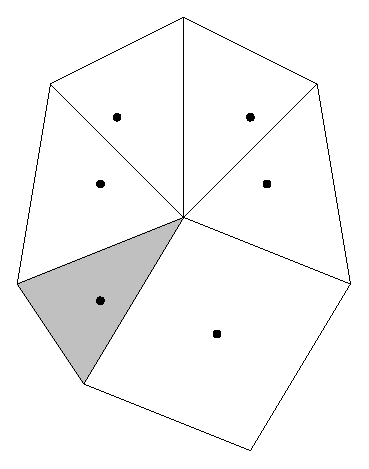
\includegraphics[width=.8\linewidth]{fig/volume_centrado.eps}
        \caption{Volume Centrado}
        \label{fig:volume_centrado}        
    \end{subfigure}
    \begin{subfigure}{.5\textwidth}
        \centering
        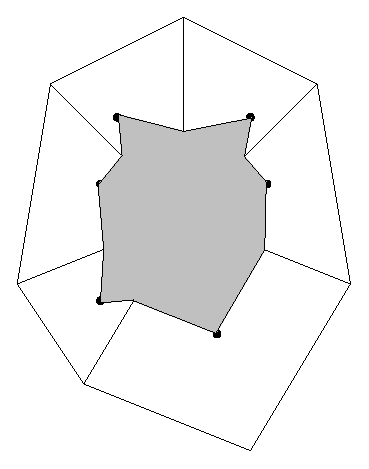
\includegraphics[width=.8\linewidth]{fig/volume_vertice.eps}
        \caption[]{Volume Baseado no vértice}
        \label{fig:volume_vertice}        
    \end{subfigure}

    \caption{Criação de Volumes de Controle}
    \label{fig:volume-controle}
\end{figure}

\section{Método dos Volumes Finitos para o problema da difusão 2D}

As equações governantes da mecânica dos fluidos, também chamadas de equações de Navier-Stokes são um conjunto de equações diferenciais que descrevem o escoamento de fluidos. Tais equações podem ser escritas de forma geral por uma equação de transporte:

\begin{equation}
    \int_{V_{CV}} \frac{\partial \rho \phi}{\partial t}dV + \int_{V_{CV}} \nabla \cdot (\rho \vec{U}\phi)dV - \int_{V_{CV}} \nabla \cdot (\rho \Gamma_\phi \nabla\phi)dV = \int_{V_{CV}} S_\phi(\phi)dV
\end{equation}

Em que $\phi$ é uma propriedade tensorial considerada contínua no espaço, $\Gamma_\phi$ é o coeficiente de difusão e $S_\phi(\phi)$ é o termo fonte. Nesse trabalho é considerado apenas o termo de difusão dessa equação, cuja discretização será apresentada a seguir.
\criarsimbolo{$ \phi $}{Propriedade Tensorial}
\criarsimbolo{$ \Gamma_\phi $}{Coeficiente de Difusão}
\criarsimbolo{$ S_\phi(\phi) $}{Termo Fonte}

O método dos volumes finitos é conservativo localmente porque ele é baseado em um balanço local escrito para cada célula de discretização, também chamada de "volume de controle". Se pegarmos uma equação de Poisson, temos que matematicamente, o lado esquerda dessa equação irá descrever um processo de difusão, enquanto que o lado direito descreve um processo de geração, por exemplo:

\begin{equation}
    \vec{q} = -k \nabla T
\end{equation}
$\vec{q}$ representa o fluxo de calor devido a diferença de temperatura
\criarsimbolo{$ \vec{q} $}{Fluxo de calor}

\begin{equation}
    \vec{J} = -D \nabla Y
\end{equation}
$\vec{J}$ representa o fluxo de massa devido a diferença de massa
\criarsimbolo{$ \vec{J} $}{Fluxo de Massa}

\begin{equation}             
    \vec{j} = -\sigma \nabla \phi
\end{equation}
$\vec{j}$ representa o fluxo de corrente devido a diferença de tensão
\criarsimbolo{$ \vec{j} $}{Fluxo de Corrente Elétrica}

Se agora, considerarmos a conservação de energia em um corpo sólido, e assumindo que:
\begin{itemize}
    \item O único modo de transferência de calor é por condução
    \item Não é realizado trabalho pelo ou sobre o sistema
    \item Estado estacionário
\end{itemize}

Nesse caso, podemos reduzir a conservação de energia em:

Taxa de transferência de calor para o volume de controle + taxa de calor gerado dentro do volume de controle = taxa de transferência de calor para fora do volume de controle.

Matematicamente, escrevemos como:

\begin{equation}
    \dot{Q_{in}} + \dot{Q_{gen}} = \dot{Q_{out}}
    \label{eq:2.4}
\end{equation}

Dado um volume $V_0$ com uma área de superfície $S$, podemos denotar $\vec{q}$ como o vetor de fluxo de calor (devido à condução) e $\vec{q} \cdot \vec{n}$ como a componente do vetor de fluxo normal a borda do volume.

Desse modo temos que $\int_S \vec{q}\cdot\hat{n}dA$ representa o total de calor sendo transferido pela fronteira do volume de controle $(\dot{Q_{out}} - \dot{Q_{in}})$ e, substituindo na equação de conservação da energia \ref{eq:2.4} temos:

\begin{equation}
    \dot{Q}_{gen} = \int_S \vec{q}\cdot\hat{n}dA = \int_V \dot{q}_{gen}dV
\end{equation}

Utilizando o teorema da divergência de Gauss podemos chegar a:

\begin{equation}
    \int_V \dot{q}_{gen}dV = \int_S \vec{q}\cdot\hat{n}dA = \int_V \nabla\cdot\vec{q}dV
\end{equation}

Combinando ambos os termos, temos:

\begin{equation}
    \int_V (\nabla \cdot \vec{q} - \dot{q}_{gen})dV = 0
\end{equation}

Como o termo dV não é igual a zero, isso implica em:

\begin{equation}
    \nabla \cdot \vec{q} - \dot{q}_{gen} = 0
    \label{difusao:poisson}
\end{equation}

Como, nesse caso o fluxo de calor é devido apenas a condução, podemos expressar ela em termos de temperatura usando a lei de Fourier da transferência de calor por condução, $\vec{q} = -k \nabla T$.

Substituindo na equação \ref{difusao:poisson} temos que:

\begin{equation}
    \nabla \cdot \vec{q} - \dot{q}_{gen} = \nabla \cdot (-k \nabla T) - \dot{q}_{gen} = 0
\end{equation}

Rearranjando:

\begin{equation}
    \nabla \cdot (k \nabla T) = -\dot{q}_{gen}
\end{equation}

Considere a seguinte equação de difusão na forma generalizada da equação de Poisson:

\begin{equation}
    \nabla \cdot (\Gamma \nabla \phi) = S_\phi
\end{equation}

Temos que $\Gamma$ é conhecido como a propriedade de transporte, e sendo um escalar, segue que:

\begin{equation}
    \Gamma \nabla \phi = \left( \Gamma \frac{\partial \phi}{\partial x} \vec{i} + \Gamma \frac{\partial \phi}{\partial y} \vec{j} + \Gamma \frac{\partial \phi}{\partial z} \vec{k} \right) = \vec{J}
\end{equation}

O fluxo é $\phi$

Segue agora que o divergente dessa expressão fica:

\begin{equation}
\begin{split}
    \nabla \cdot (\Gamma \nabla \phi) &= \left( \frac{\partial}{\partial x}\vec{i} + \frac{\partial}{\partial y}\vec{j} + \frac{\partial}{\partial z}\vec{k} \right) \cdot \left( \Gamma \frac{\partial \phi}{\partial x}\vec{i} + \Gamma \frac{\partial \phi}{\partial y}\vec{j} + \Gamma \frac{\partial \phi}{\partial z}\vec{k} \right)\\
    &= \frac{\partial}{\partial x} \left( \Gamma \frac{\partial \phi}{\partial x} \right) + \frac{\partial}{\partial y} \left( \Gamma \frac{\partial \phi}{\partial y} \right) + \frac{\partial}{\partial z} \left( \Gamma \frac{\partial \phi}{\partial z} \right)
\end{split}
\end{equation}

Portanto, a equação inicial, em coordenadas cartesianas, pode ser escrita como:

\begin{equation}
    \frac{\partial}{\partial x} \left( \Gamma \frac{\partial \phi}{\partial x} \right) + \frac{\partial}{\partial y} \left( \Gamma \frac{\partial \phi}{\partial y} \right) + \frac{\partial}{\partial z} \left( \Gamma \frac{\partial \phi}{\partial z} \right) = S_\phi
\end{equation}

No método dos volumes finitos, deve-se integrar a equação governante sobre um volume de controle antes de se fazer as aproximações das derivadas. Desse modo temos:

\begin{equation}
    \int_{V_0} \nabla \cdot (\Gamma \nabla \phi) dV = \int_{V_0} S_\phi dV
\end{equation}

Se agora aplicarmos o teorema da divergência de Gauss no lado esquerdo dessa equação, temos:

\begin{equation}
    \int_{V_0} \nabla \cdot (\Gamma \nabla \phi) dV = \int_{V_0} \nabla \cdot (\vec{J}) dV = \int_S \vec{J} \cdot \hat{n} dA
\end{equation}

Sendo $\vec{J}$ um vetor de fluxo e $\hat{n}$ é um vetor normal que aponta para fora do elemento de área $dA$.

No método de volumes finitos, todas as informações são armazenadas no centro das células.

Uma hipótese crítica que deve ser aceita, é a de que o valor da quantidade analisada nesse interior da célula é igual a média dessa quantidade em todo o volume.

Sob essa hipótese, temos que a média de $S_\phi$ no volume pode ser adquirida com o seu valor no centro da célula, portanto:

\begin{equation}
    \int_{V_0} S_\phi dV \approx S_{\phi,0} V_0
\end{equation}

O resultado final da expressão é dado por:

\begin{equation}
    \int_S (\Gamma \nabla \phi) \cdot \hat{n} dA = S_{\phi,0} V_0
\end{equation}

Essa equação para volumes finitos é válida para um volume de controle de formato arbitrário, nota-se que essa é na verdade uma equação integral e portanto é chamada de forma fraca da equação.

No contexto da resolução desse método computacionalmente, temos que os volumes de controle são limitados por um número finito de faces planas (em 3D) ou de faces lineares (em 2D). Portanto temos que a integral pode ser substituida por uma soma discreta sobre essas faces, resultando em:

\begin{equation}
    \sum_f \vec{J} \cdot \hat{n}_f A_f = \sum_f \Gamma_f (\nabla \phi)_f \cdot \hat{n}_f A_f = S_{\phi,0} V_0
\end{equation}

Nota-se que não é feita nenhuma consideração com relação ao formato ou tamanho do volume de controle.

De modo a continuar com a discretização da equação, deve-se aproximar o gradiente de $\phi$ em termos dos valores de $\phi$ no centro da célula, para isso usa-se a seguir um exemplo de um pedaço de uma malha como na figura \ref{fig:fig1}.

Considerando a malha da figura \ref{fig:fig1}, tem-se que a equação expandida fica como:

\begin{figure}
    \centering
    \caption{Grade para o FVM}
    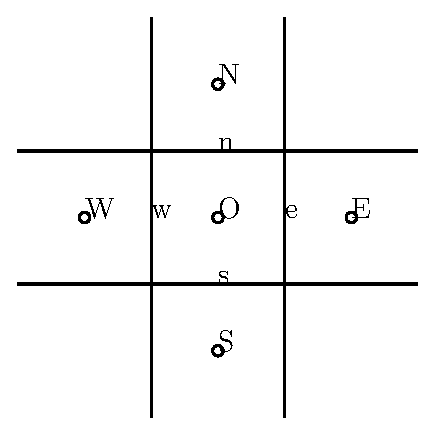
\includegraphics{fig/figura1}
    \label{fig:fig1}    
\end{figure}

\begin{equation}
    \Gamma_e (\nabla \phi)_e \cdot \hat{n}_e A_e + \Gamma_w (\nabla \phi)_w \cdot \hat{n}_w A_w + \Gamma_n (\nabla \phi)_n \cdot \hat{n}_n A_n + \Gamma_s (\nabla \phi)_s \cdot \hat{n}_s A_s = S_{\phi,0} V_0
\end{equation}

Para essa malha, temos que:

\begin{eqnarray}
    V_0 =& \Delta x \Delta y\\
    A_e =& A_w = \Delta y\\
    A_n =& A_s = \Delta x
\end{eqnarray}

Também podemos dizer:

\begin{eqnarray}
    \hat{n}_e =& \hat{i}\\
    \hat{n}_w =& -\hat{i}\\
    \hat{n}_n =& \hat{j}\\
    \hat{n}_s =& -\hat{j}
\end{eqnarray}

Considerando a definição de gradiente, chegamos a:

\begin{equation}
    (\nabla \phi)_e \cdot \hat{n}_e = \left( \frac{\partial \phi}{\partial x} \hat{i} + \frac{\partial \phi}{\partial y} \hat{j} + \frac{\partial \phi}{\partial z} \hat{k} \right) \cdot \hat{i} = \left( \frac{\partial \phi}{\partial x} \right)_e
\end{equation}

Temos um termo similar para os outros três termos.

Logo a equação governante fica como:

\begin{equation}
    \label{eq:2.29}
    \Gamma_e \left( \frac{\partial \phi}{\partial x} \right)_e \Delta y - \Gamma_w \left( \frac{\partial \phi}{\partial x} \right)_w \Delta y + \Gamma_n \left( \frac{\partial \phi}{\partial x} \right)_n \Delta x - \Gamma_s \left( \frac{\partial \phi}{\partial x} \right)_e \Delta x = S_{\phi,0} \Delta x \Delta y
\end{equation}

O próximo passo é expressar as quantidades nas faces (e,w,n,s) em termos das quantidades nos centros das células (E,W,N,S).

Normalmente, de modo a se obter o coeficiente de transporte nas faces, usa-se uma interpolação linear, para uma malha uniforme para a face e, fica como:

\begin{equation}
    \Gamma_e = \frac{\Gamma_E + \Gamma_O}{2}
\end{equation}

Para expressar a derivada de primeira ordem em termos de valores no centro das células, é empregado a expansão em série de Taylor:

\begin{equation}
    \label{eq:8}
    \phi_E = \phi_e + \frac{\Delta x}{2} \frac{\partial \phi}{\partial x} \bigg|_e + \frac{(\Delta x / 2)^2}{2!} \frac{\partial^2 \phi}{\partial x^2} \bigg|_e + \frac{(\Delta x / 2)^3}{3!} \frac{\partial^3 \phi}{\partial x^3} \bigg|_e + ...
\end{equation}

\begin{equation}
    \label{eq:9}
    \phi_O = \phi_e - \frac{\Delta x}{2} \frac{\partial \phi}{\partial x} \bigg|_e + \frac{(\Delta x / 2)^2}{2!} \frac{\partial^2 \phi}{\partial x^2} \bigg|_e - \frac{(\Delta x / 2)^3}{3!} \frac{\partial^3 \phi}{\partial x^3} \bigg|_e + ...
\end{equation}

Subtraindo \ref{eq:9} de \ref{eq:8} chegamos a:

\begin{equation}
    \label{eq:10}
    \phi_E - \phi_O = \Delta x \frac{\partial \phi}{\partial x} \bigg|_e + \frac{(\Delta x / 2)^3}{3} \frac{\partial^3 \phi}{\partial x^3} \bigg|_e + ...
\end{equation}

Rearranjando a equação \ref{eq:10} chegamos no chamado "Central Difference scheme":

\begin{equation}
    \label{eq:11}
    \frac{\partial \phi}{\partial x} \bigg|_e = \frac{\phi_E - \phi_O}{\Delta x} - \frac{(\Delta x)^2}{24} \frac{\partial^3 \phi}{\partial x^3} \bigg|_e + ...
\end{equation}

Nota-se que essa aproximação é de segunda ordem.

Substituindo a expressão para a aproximação numérica da derivada de primeira ordem e os coeficientes de transporte na equação governante discretizada pelo método dos volumes finitos temos:

\begin{equation}
    \begin{split}
    \label{eq:12}
    &\frac{\Gamma_E + \Gamma_O}{2} \left( \frac{\phi_E - \phi_O}{\Delta x} \right) \Delta y - \frac{\Gamma_W + \Gamma_O}{2} \left( \frac{\phi_O - \phi_W}{\Delta x} \right) \Delta y + \frac{\Gamma_N + \Gamma_O}{2} \left( \frac{\phi_N - \phi_O}{\Delta y} \right) \Delta x\\
    &- \frac{\Gamma_S + \Gamma_O}{2} \left( \frac{\phi_O - \phi_S}{\Delta y} \right) \Delta x = S_{\phi,0} \Delta x \Delta y
    \end{split}
\end{equation}

A equação \ref{eq:12} pode ser reescrita em um formato que irá gerar uma matriz penta-diagonal no seguinte formato:

\begin{equation}
    a_P \phi_P = a_W \phi_W + a_E \phi_E + a_N \phi_N + a_S \phi_S - b_P
\end{equation}

Cujos coeficientes são:

\begin{eqnarray}
    a_P =& \left( \frac{\Gamma_E + \Gamma_O}{2 \Delta x} \Delta y + \frac{\Gamma_W + \Gamma_O}{2 \Delta x} \Delta y + \frac{\Gamma_N + \Gamma_O}{2 \Delta y} \Delta x + \frac{\Gamma_S + \Gamma_O}{2 \Delta y} \Delta x \right)\\
    a_E =& \frac{\Gamma_E + \Gamma_O}{2 \Delta x} \Delta y\\
    a_W =& \frac{\Gamma_W + \Gamma_O}{2 \Delta x} \Delta y\\
    a_N =& \frac{\Gamma_N + \Gamma_O}{2 \Delta y} \Delta x\\
    a_S =& \frac{\Gamma_S + \Gamma_O}{2 \Delta y} \Delta x\\
    b_P =& S_{\phi,0} \Delta x \Delta y
\end{eqnarray}

Se for considerado uma condição de contorno de Dirichlet, teremos, conforme a seguinte figura onde $w$ é conhecido:

\begin{figure}[h!]
    \centering
    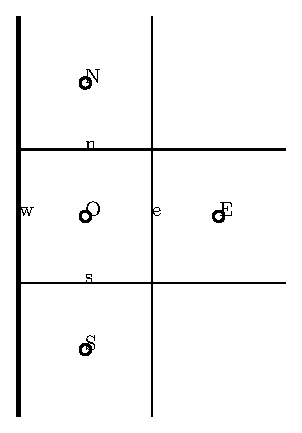
\includegraphics[width=0.4\linewidth]{fig/figura2.eps}
    \caption{Condições de contorno}
    \label{fig:fig2}
\end{figure}

Nesse caso teremos que a aproximação numérica da derivada com relação a face $w$ não pode mais ser feita com CDS-2 pois não existe outra célula a oeste dessa.

Pode-se então usar a aproximação DDS-4 para essa derivada de modo a manter a equação com um erro de segunda ordem.

\begin{equation}
    \label{eq:2.43}
    \frac{\partial \phi}{\partial x} \bigg|_w = \frac{9 \phi_O - \phi_{E} -8\phi_w}{3 \Delta x} + \frac{(\Delta x)^2}{9} \frac{\partial^3 \phi}{\partial x^3} \bigg|_w + ...
\end{equation}

Substituindo agora a equação \ref{eq:2.43} que é a expressão para a derivada do fluxo em relação a $x$ na face $w$ na equação \ref{eq:2.29} tem-se:

\begin{equation}
    \label{eq:2.44}
    \left\{ \Gamma \frac{\partial \phi}{\partial x}\bigg|_e -\Gamma \frac{\partial \phi}{\partial x}\bigg|_w  \right\} \Delta y + \left\{\Gamma \frac{\partial}{\partial y}\bigg|_n - \Gamma \frac{\partial \phi}{\partial y}\bigg|_s  \right\} \Delta x = S_{\phi,o}\Delta x \Delta y
\end{equation}

\begin{equation}
    \label{eq:2.45}
    \left\{\Gamma_e \frac{\Phi_E-\Phi_O}{\Delta x} - \Gamma_w \frac{9 \phi_O - \phi_{E} -8\phi_w}{3 \Delta x} \right\} \Delta y + \left\{\Gamma_n \frac{\Phi_N-\Phi_O}{\Delta y} - \Gamma_s \frac{\Phi_O-\Phi_S}{\Delta y}  \right\} \Delta x = S_{\phi,o}\Delta x \Delta y
\end{equation}

Rearranjando-se a equação \ref{eq:2.45} e aplicando a condição de contorno $\phi_w = \phi_{left}$ temos:

\begin{equation}
\begin{split}
    &\left[\left( \frac{\Gamma_e}{\Delta x}+\frac{3\Gamma_w}{\Delta x}\right)\Delta y  + \left(\frac{\Gamma_n}{\Delta y}+\frac{\Gamma_w}{\Delta y}\right)\Delta x  \right]\phi_O\\
    - &\left[\left(\frac{\Gamma_e}{\Delta x}+\frac{\Gamma_w}{3\Delta x}\right)\Delta y\right]\phi_E\\
    - & \left[\left(\frac{\Gamma_n}{\Delta y}\right)\Delta x\right]\phi_N-\left[\left(\frac{\Gamma_s}{\Delta y}\right)\Delta x\right]\phi_S = S_{\phi,o}\Delta x \Delta y + \left[\frac{8\Gamma_w \Delta y}{3 \Delta x}\right]\phi_w
\end{split}
\end{equation}

Nesse caso teremos que a matriz da equação com relação a essa condição de contorno continuará sendo penta-diagonal, e a informação da condição de contorno ficará no termo fonte correspondente.

Já para o caso da condição de contorno de Neumann, teremos apenas que substituir na equação \ref{eq:2.29} o valor para o fluxo correspondente que já é conhecido.

\section{Análise de erros no método dos volumes finitos}

Na solução do FVM temos que considerar o erro de discretização gerado, essa estimativa de erro já foi realizado várias vezes e existe na literatura como em \cite{Jasak1996} e \cite{Muzaferija2014}.

Segundo \cite{Juretic2004} tanto a qualidade da malha quanto o formato da célula utilizado influenciam na acurácia da solução, que varia para o termo convectivo e difusivo da equação diferencial a ser solucionada.

Na discretização do método dos volumes finitos, uma importante propriedade necessária dessa discretização é que a solução encontrada deve tender à solução exata dado que o número de volumes de controle tenda ao infinito. Para isso ocorrer deve-se satisfazer os seguintes requisitos:
\begin{itemize}
    \item \textbf{Consistência:} O erro de discretização na solução numérica deve tender a zero a medida que o espaçamento da malha tenda a zero.
    \item \textbf{Estabilidade:} A discretização é considerada estável se ela não aumenta nenhum erro durante o processo de cálculo.
    \item \textbf{Concervação:} O FMV é obtido com a integração da equação diferencial governante e, portanto, para propriedades conservativas deve obedecer às mesmas leis de conservação da equação diferencial.
    \item \textbf{Limitação:} Algumas propriedades físicas ficam entre certas fronteiras, por exemplo a densidade nunca é negativa, logo deve-se ter como requisito que a discretização não gere valores impossíveis na física.
\end{itemize}
\cite{Juretic2004}

Nese trabalho é considerado apenas as malhas 2D com o formato de célula triangular pois este é muito comum e mais facilmente implementado, outra limitação desse trabalho é que é considerado apenas o termo difusivo.

Conforme foi mostrado, a partir da equação \ref{eq:2.29}, as derivadas dessa equação são aproximadas usando-se a geometria da malha, no caso com uma célula quadrada. Logo tem-se que o formato da célula influencia na acurácia da solução. A partir da geometria da malha, pode-se gerar as seguintes propriedades:

\begin{itemize}
    \item \textbf{Não Ortogonalidade:} Conforme a figura \ref{nao-ortogo} pode-se definir a não Ortogonalidade como o angulo $\theta$ entre o vetor $d=\vec{PA}$ e o vetor normal a face ab $\hat{n}$. Esse angulo deve ser o menor possível. A razão será discutida posteriormente.
    \item \textbf{Assimetria de malha:} Quando o vetor d não intercepta a face ab no seu centro, a célula de malha é definida como assimétria conforme a figura \ref{fig:assimetria}. O grau de assimetria pode ser definido como $\Psi = \frac{|m|}{|d|}$
    \item \textbf{Uniformidade:}  Uma malha é uniforme quando o vetor $\vec{d}$ intercepta a face no meio entre os nós $P$ e $N$. A uniformidade pode ser medida como:
    \begin{equation*}
        f_x = \frac{|x_{fi}-x_N|}{|d|}
    \end{equation*}
    portanto $f_x=0.5$ é o valor para uma malha uniforme. Esta propriedade afeta a acurácia dos termos de gradiente.
\end{itemize}

\begin{figure}
    \begin{subfigure}{.5\textwidth}
        \centering
        \caption{Não Ortogonalidade}
        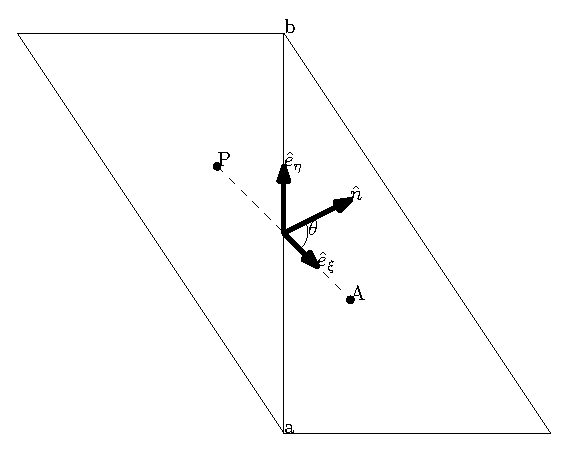
\includegraphics[width=.8\linewidth]{fig/nao-ortogo}
        \label{nao-ortogo}
    \end{subfigure}
    \begin{subfigure}{.5\textwidth}
        \centering
        \caption{Assimetria}
        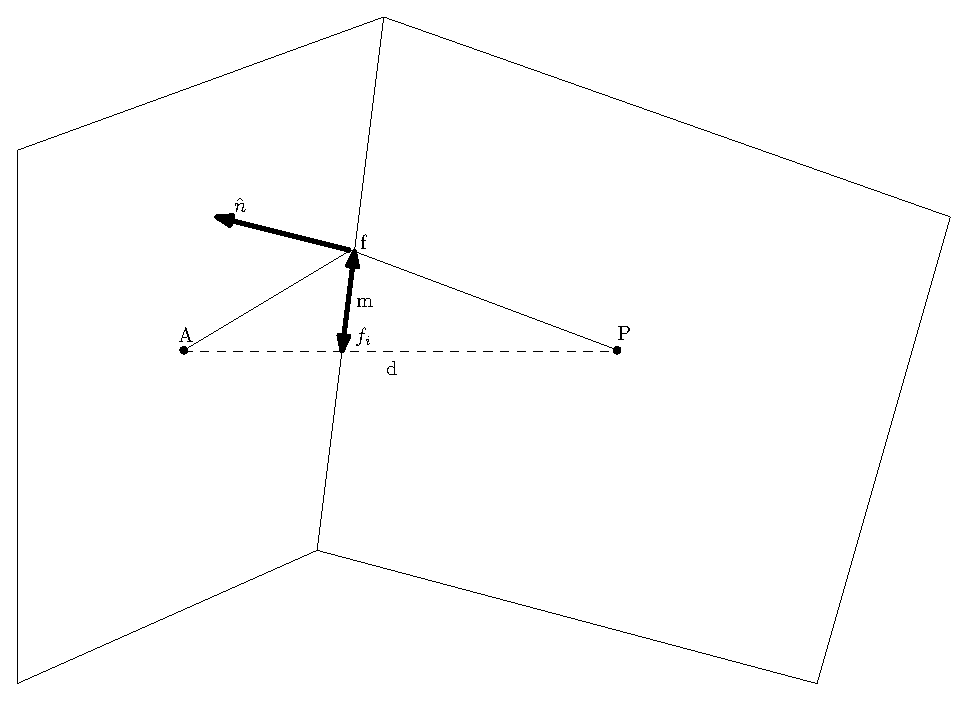
\includegraphics[width=.8\linewidth]{fig/assimetria.eps}
        \label{fig:assimetria}
    \end{subfigure}

    \caption{Erros no volume finito}
\end{figure}

\section{Termo de Difusão}

A partir da equação \ref{eq:2.1} considerando-se o termo de difusão, aplicando-se o teorema da divergência de Gauss e a aproximação de que os gradientes nas faces são constantes (assumindo-se uma variação linear da propriedade $\phi$) chega-se a:

\begin{equation}
    \int_{V_P} \nabla \cdot (\rho \Gamma_\phi \nabla\phi)dV = \sum_f \vec{S} \cdot (\rho \Gamma_\phi \nabla \phi)_f = \sum (\rho \Gamma_\phi)_f (\vec{S} \cdot \nabla \phi)_f
\end{equation}

Onde o vetor $\vec{S}$ está na figura \ref{fig:non-orthogonality}

\begin{figure}[]
    \centering
    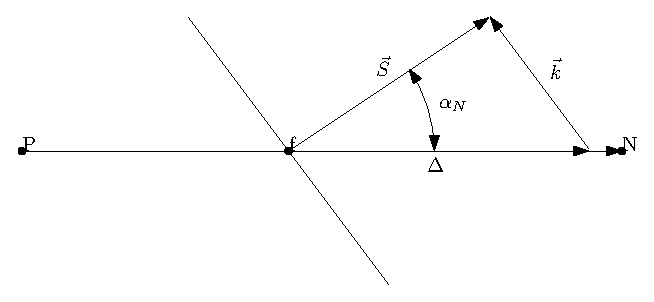
\includegraphics{fig/non-orthogonality.eps}
    \caption{Erro do termo difusivo em malha não ortogonal}
    \label{fig:non-orthogonality}
\end{figure}

% O termo $(\rho \Gamma_\phi)_f$ é interpolado nas faces usando-se a equação \ref{eq:2.49}. Onde $\phi_{f_i}$ e $(\nabla \phi)_{f_i}$ são os valores de $\phi$ e $\nabla \phi$ no ponto onde o vetor $\vec{d}$ intercepta a face conforme a figura \ref{fig:assimetria}.

% \begin{equation}
%     \phi_f = \phi_{f_i} = \vec{m} \cdot (\nabla \phi)_{f_i}
%     \label{eq:2.49}
% \end{equation}

% Já o termo $(\vec{S} \cdot \nabla \phi)_f$ é aproximado usando-se a seguinte equação:

% \begin{equation}
%     (\vec{S} \cdot \nabla \phi)_f = 
% \end{equation}

Segundo a dedução encontrada em \cite{Juretic2004} a ordem do erro do termo de difusão é igual a menor entre a ordem do erro de interpolação e do erro de discretização do termo gradiente dados por:

\begin{equation}
    e_{interpolation} = -\frac{1}{2} |\vec{d^2}| (f_x(1-f_x)(\hat{d^2}:(\nabla \nabla \phi)_{f_i} + \psi |\vec{d}| \hat{m} \cdot (\hat{d^2} : (\nabla \nabla \nabla \phi)_{f_i})) + \frac{\psi^2}{2} |\vec{d^2}| (\hat{m^2} : (\nabla \nabla \phi)_{f_i}) )
    \label{eq:2.49}
\end{equation}

\begin{equation}
    e_{snGrad} = -\frac{|\vec{S}|}{6 \cot{\alpha_N}} |\vec{d^2}| ((1-f_x)^3 + f_x^3)\hat{d^3}:: (\nabla \nabla \nabla \phi)_f - |\vec{S}| \tan{\alpha_N} \frac{|\vec{d^2}|}{2}f_x(1-f_x)\hat{k} \cdot (\hat{d^2}:(\nabla \nabla \nabla \phi)_f)
    \label{eq:2.50}
\end{equation}

Onde $\hat{d}$ e $\hat{k}$ são vetores unitários nas direções de $\vec{d}$ e $\vec{k}$ respectivamente. Verifica-se da equação \ref{eq:2.50} que essa será de primeira-ordem com exceto para o falor de $f_x=0.5$, ou seja, para uma malha uniforme. Logo para uma malha uniforme a aproximação se torna de segunda-ordem. O erro também depende do ângulo $\alpha_N$ e será mínimo quando $\alpha_N=0$, ou seja, quando a malha for ortogonal.